\chapter{Ergebnisse}

\section{Klassische Metriken}

In den Tabellen \ref{tab:eventweise 1} und \ref{tab:eventweise 2} wird der in dieser Arbeit implementierte Detektor mit den Detektoren aus der Literatur anhand eventweise berechneter klassischen Metriken verglichen. Zu beachten ist, dass der Detektor größtenteils aus der Veröffentlichung von Moore et al. \cite{Moore} übernommen wurde.
In der Statistik wurden Annotationen ausgeschlossen, bei denen die jeweilige Metrik unendlich wurde.
Die Mittelwerte werden stark durch die große Abweichung weniger Extremfälle beeinflusst. Um die Verteilung besser zu repräsentieren wurde zusätzlich der Median angegeben.


\begin{table}[!ht]
    \caption{Stand der Technik für eventweise Auswertung zur Einordnung des implementierten Detektors, Teil 1; Der Zusatz 'r' bezeichnet einen rekonstruierten Wert}   
	\centering
		\begin{tabular}{llllllllll}
			\hline & \cite{Huang} & \cite{Moore} & \cite{Moore} & \cite{alvarez} & \cite{ferri}\\
			\hline {$\!\begin{aligned}
				&\\
			    Datensatz\\
			    Art\ des\ Klassifikators\\
			    Berechnungsart\\
			    \gls{Sens}\\
			    \gls{Prec}\\
			    \gls{Spez}\\
			    \gls{NPV}\\
			    \gls{Acc}\\
			    Cohens\ \kappa\\
			    F1-Ma"s\\
			    Korrealtion\ PLM/h\\
			    relative\ \#\ PLM\\
				&\\
				\end{aligned}$} & {$\!\begin{aligned}
				&\\
				15\ \gls{RLS}\ (24)\\
				statisch\\
				Event\\
				0.95\\
				-\\
				0.92\\
				-\\
				-\\
				-\\
				0.93r\\
				0.97\\
				1\\
				&\\
				\end{aligned}$} & {$\!\begin{aligned}
				&\\
				\acrshort{WSC}\ (1073)\\
				dynamisch\\
			    Event\ \cite{git}\\
				0.6\\
				0.88\\
				1\\
				0.99\\
				0.98\\
				0.71\\
				-\\
				0.94\\
				0.63\\
				&\\
				\end{aligned}$} & {$\!\begin{aligned}
				&\\
				\acrshort{SSC}\ (760)\\
				dynamisch\\
				Event\ \cite{git}\\
				0.75\\
				0.82\\
				1\\
				0.99\\
				0.99\\
				0.87\\
				-\\
				0.94\\
				0.92\\
				&\\
				\end{aligned}$}  & {$\!\begin{aligned}
				&\\
			    \acrshort{HMC}\ (70)\\
				dynamisch\\
				Segment\ (1s)\\
				0.82\\
				0.71\\
				1\\
				-\\
				1\\
				0.73\\
				0.73\\
				-\\
				0.99\\
				&\\
				\end{aligned}$}  & {$\!\begin{aligned}
				&\\
				\acrshort{WSC}\ (60)\\
				statisch.\\
				Event\\
				0.85\\
				0.62\\
				0.99\\
				1\\
				0.99\\
				0.72\\
				-\\
				-\\
				1.3\\
				&\\
				\end{aligned}$}
				\\
				\hline
		\end{tabular}

\label{tab:eventweise 1}
\end{table}


\begin{table}[!ht]
    \caption{Stand der Technik für eventweise Auswertung zur Einordnung des implementierten Detektors, Teil 2}   
	\centering
		\begin{tabular}{lllllllllll}
			\hline & \cite{wetter} & \cite{Carvelli}& \cite{Carvelli}& \cite{Carvelli}& implement. Detektor\\
			\hline {$\!\begin{aligned}
			    &\\
			    Datensatz\\
			    Klassifikatorart\\
			    Berechnungsart\\
			    \gls{Sens}\\
			    \gls{Prec}\\
			    \gls{Spez}\\
			    \gls{NPV}\\
			    \gls{Acc}\\
			    Cohens\ \kappa\\
			    F1-Ma"s\\
			    Korrealtion\ PLM/h\\
			    relative\ \#\ PLM\\
				&\\
				\end{aligned}$} & {$\!\begin{aligned}
				&\\
				\acrshort{WSC}\ (60)\\
				statisch\\
				Event\\
				0.96\\
				0.47\\
				0.98\\
				1\\
				0.98\\
				0.62\\
				-\\
				-\\
				2\\
				&\\
				\end{aligned}$} & {$\!\begin{aligned}
				&\\
                \acrshort{WSC}\ (275)\\
				\acrshort{DNN}\\
				Event\\
				0.9\\
				0.81\\
				-\\
				-\\
				-\\
				-\\
				0.83\\
				-\\
				-\\
				&\\
				\end{aligned}$}& {$\!\begin{aligned}
				&\\
                \acrshort{SSC}\ (177)\\
				\acrshort{DNN}\\
				Event\\
				-\\
				-\\
				-\\
				-\\
				-\\
				-\\
				0.71\\
				-\\
				-\\
				&\\
				\end{aligned}$}& {$\!\begin{aligned}
				&\\
                \acrshort{MrOS}\ (348)\\
				\acrshort{DNN}\\
				Event\\
				-\\
				-\\
				-\\
				-\\
				-\\
				-\\
				0.77\\
				-\\
				-\\
				&\\
				\end{aligned}$} & {$\!\begin{aligned}
				&\\
                Uniklinik\ DD\ (5908)\\
                dynamisch\\
				Event\\
				0.6\\
				0.68\\
				0.84\\
				0.78\\
				0.72\\
				0.41\\
				0.57\\
    			0.48\\
    			1.4\\
				&\\
				\end{aligned}$}
				\\
				\hline
		\end{tabular}

\label{tab:eventweise 2}
\end{table}

In Tabelle \ref{tab:segemtnweise} ist gesondert der Vergleich der segmentweisen Auswertung zu sehen. Zu beachten ist, dass in dem implementierten Detektor besonders die Metriken einen hohen Wert aufweisen, die ein \gls{TN} im Zähler haben.
\begin{table}[!ht]
    \caption{Stand der Technik für segmentweise Auswertung zur Einordnung des implementierten Detektors}   
	\centering
		\begin{tabular}{lll}
			\hline & \cite{alvarez} & implement. Detektor\\
			\hline {$\!\begin{aligned}
			    &\\
			    Datensatz\\
			    Klassifikatorart\\
			    Berechnungsart\\
			    \gls{Sens}\\
			    \gls{Prec}\\
			    \gls{Spez}\\
			    \gls{NPV}\\
			    \gls{Acc}\\
			    Cohens\ \kappa\\
			    F1-Ma"s\\
			    Korrealtion\ PLM/h\\
			    relative\ \#\ PLM\\
				&\\
				\end{aligned}$} & {$\!\begin{aligned}
				&\\
				\acrshort{HMC}\ (70)\\
				dyn.\\
				Segment\ (1s)\\
				0.82\\
				0.71\\
				1\\
				-\\
				1\\
				0.73\\
				0.73\\
				-\\
				0.99\\
				&\\
				\end{aligned}$} & {$\!\begin{aligned}
				&\\
                Uniklinik\ DD\ (5908)\\
                dyn.\\
				Segment\ (1s)\\
				0.49\\
			    0.6\\
				0.99\\
			    0.98\\
				0.97\\
				0.46\\
				0.47\\
    			0.48\\
    			1.4\\
				&\\
				\end{aligned}$}
				\\
				\hline
		\end{tabular}

\label{tab:segemtnweise}
\end{table}


\section{Kostenfunktional}
\begin{table}[!ht]
    \caption{Korrelation zwischen Kostenfunktional und klassischen Metriken}
	\centering
		\begin{tabular}{llllllll}
			\hline & F1-Ma"s& Cohens $\kappa$ & \gls{Spez} & \gls{Prec} & \gls{Sens}& \gls{Acc}& \gls{NPV}\\
			\hline {$\!\begin{aligned}
				&\\
				Kostenfunktional\\
				&\\
				\end{aligned}$} & {$\!\begin{aligned}
				&\\
			    -0.184\\
				&\\
				\end{aligned}$}& {$\!\begin{aligned}
				&\\
			    -0.125\\
				&\\
				\end{aligned}$}& {$\!\begin{aligned}
				&\\
			    0.251\\
				&\\
				\end{aligned}$}& {$\!\begin{aligned}
				&\\
			    0.175\\
				&\\
				\end{aligned}$}& {$\!\begin{aligned}
				&\\
			    -0.262\\
				&\\
				\end{aligned}$}& {$\!\begin{aligned}
				&\\
			    -0.159\\
				&\\
				\end{aligned}$}& {$\!\begin{aligned}
				&\\
			    -0.283\\
				&\\
				\end{aligned}$}\\
			    \hline
		\end{tabular}

\label{tab:KorrMetriken}
\end{table}


Das Kostenfunktional korreliert nur schwach mit den klassischen Metriken (siehe Tabelle \ref{tab:KorrMetriken}).

Die Tabelle \ref{tab:Kostenbeiträge} schlüsselt die Beiträge der verschiedenen Fehler zu der Gesamtkostenzahl auf.
Zur besseren Einordnung der Mittelwerte sind zusätzlich noch die Anzahl der Annotationen aufgelistet, die keine Kosten verursacht haben. Die relativen Kosten sind definiert durch die absoluten Kosten bezogen auf die manuelle PLM Anzahl.
An dieser Aufschlüsselung der Kosten ist interessant, dass wenig Fehler durch Xto1- und 1toX- Matches entstanden sind.
Die Hauptfehlerquelle ist eine Verminderung der PLM Anzahl aufgrund von \gls{FN} (41 Prozent).

\begin{table}[!ht]
\caption{Beiträge der Fehlerarten an den Gesamtkosten. (+) hinter der Fehlerart beschreibt, dass dieser Fehler zu einer Erhöhung des PLM-Indexes geführt hat. (-) steht analog für eine Verminderung.}
	\centering
		\begin{tabular}{lll}
			\hline Fehlerart & Mittelwert & \# Dateien ohne Kosten\\
			\hline {$\!\begin{aligned}
				&\\
				FP\ (+)\\
				1toX\ (+)\\
				Zeitungenauigkeiten\ (+)\\
				FN\ (-)\\
    			Xto1\ (-)\\
				Zeitungenauigkeiten\ (-)\\
				absolute\ Kosten\\
				relative\ Kosten\\
			
				&\\
				\end{aligned}$} & {$\!\begin{aligned}
				&\\
				42\\
				1.25\\
				72\\
				117\\
				2.05\\
				72.9\\
				285\\
				2.26\\
				&\\
				\end{aligned}$} & {$\!\begin{aligned}
				&\\
				1341\\
				4718\\
				1108\\
				873\\
				4274\\
				988\\
				488\\
				488\\
				&\\
				\end{aligned}$}\\
				\hline
		\end{tabular}

\label{tab:Kostenbeiträge}
\end{table}


Die Differenz aus ergebniserhöhenden Fehlern und ergebnisvermindernden Fehlern ($K_{diff}$) korreliert gut mit der Differenz aus automatisch annotierten PLM und manuell annotierten PLM (siehe Bild \ref{fig:plotKorr}). Der Korrelationskoeffizient liegt bei 0.987. Dieser Wert beschreibt den Zusammenhang zwischen den erklärten Fehlern aus dem Kostenfunktional und dem medizinisch wichtigen PLM-Index.


Die Verteilugen der absoluten und relative Kosten (absolute Kosten bezogen auf die manuelle PLM-Anzahl) sind in Abb. \ref{fig:Kostennebeneinander} dargestellt. Es ist zu erkennen, dass Annotationen an denen höhere Kosten entstanden sind, seltener sind. 

\begin{figure}[!ht]%
	\begin{center}
	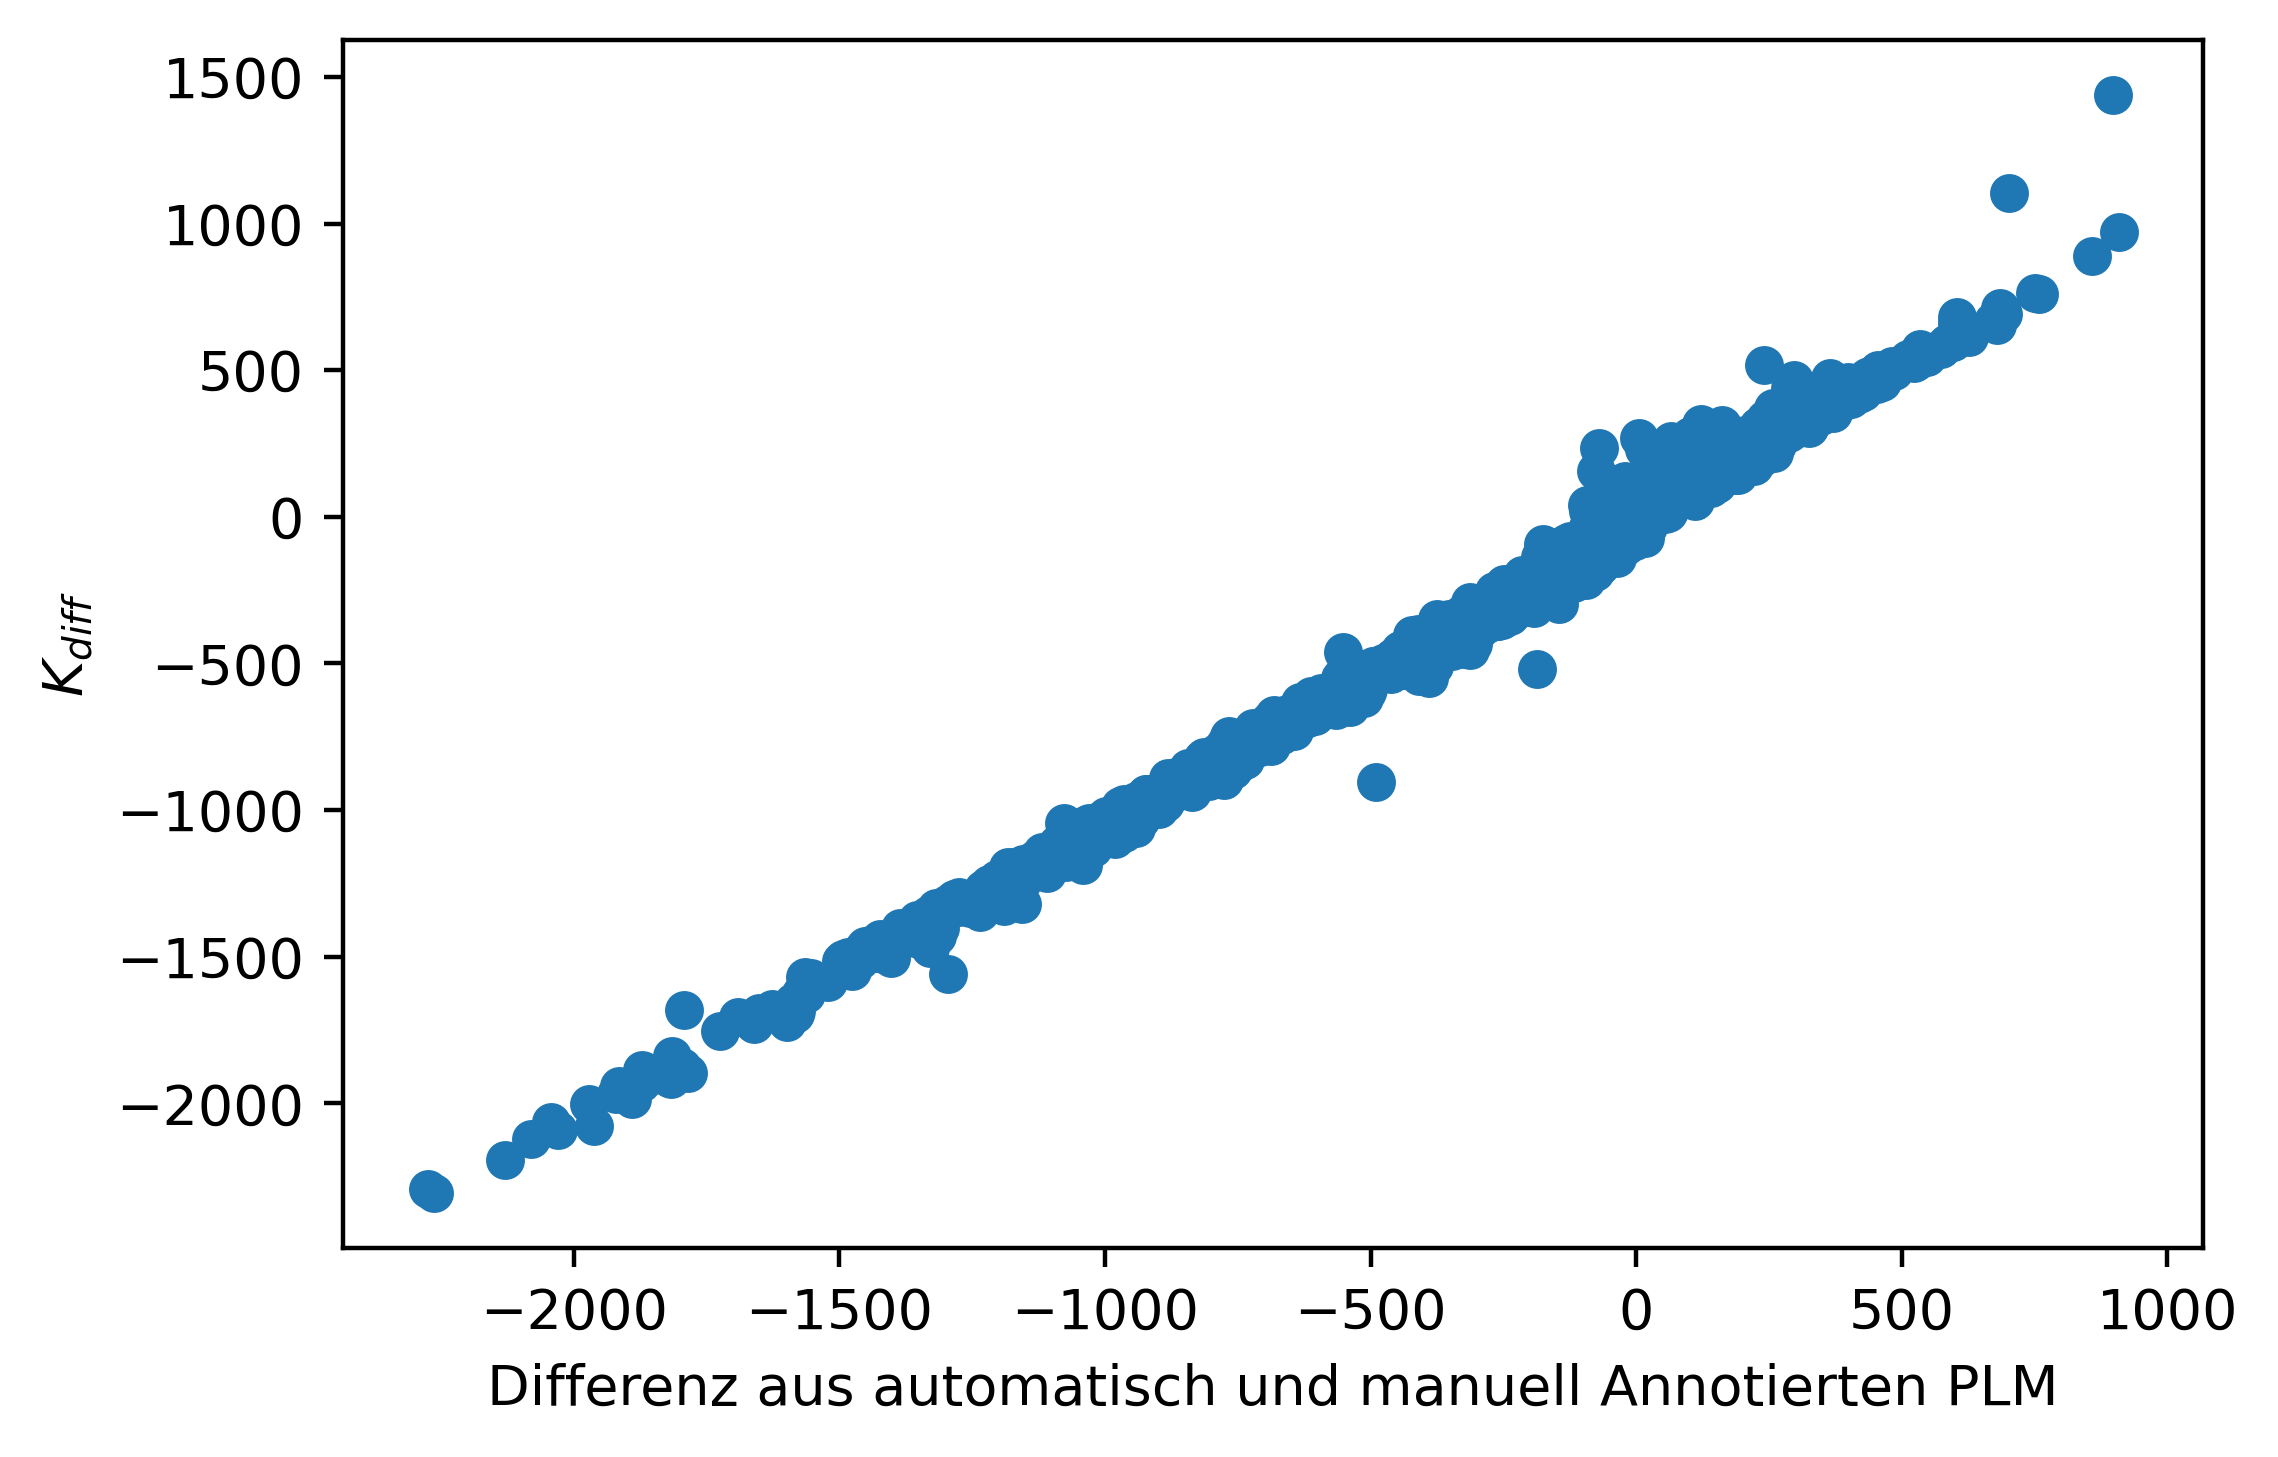
\includegraphics[width=0.80\textwidth]{./Bilder/korre.png}
	\end{center}
	\caption{Veranschaulichung der Korrelation von Differenz aus ergebniserhöhenden Fehlern und ergebnisvermindernden Fehlern ($K_{diff}$) und Differenz aus automatisch annotierten und manuell annotierten PLM.}%
	\label{fig:plotKorr}%
\end{figure}

\begin{figure}[!ht]%
\centering
	\begin{subfigure}[t]{.49\linewidth}%
		\centering
		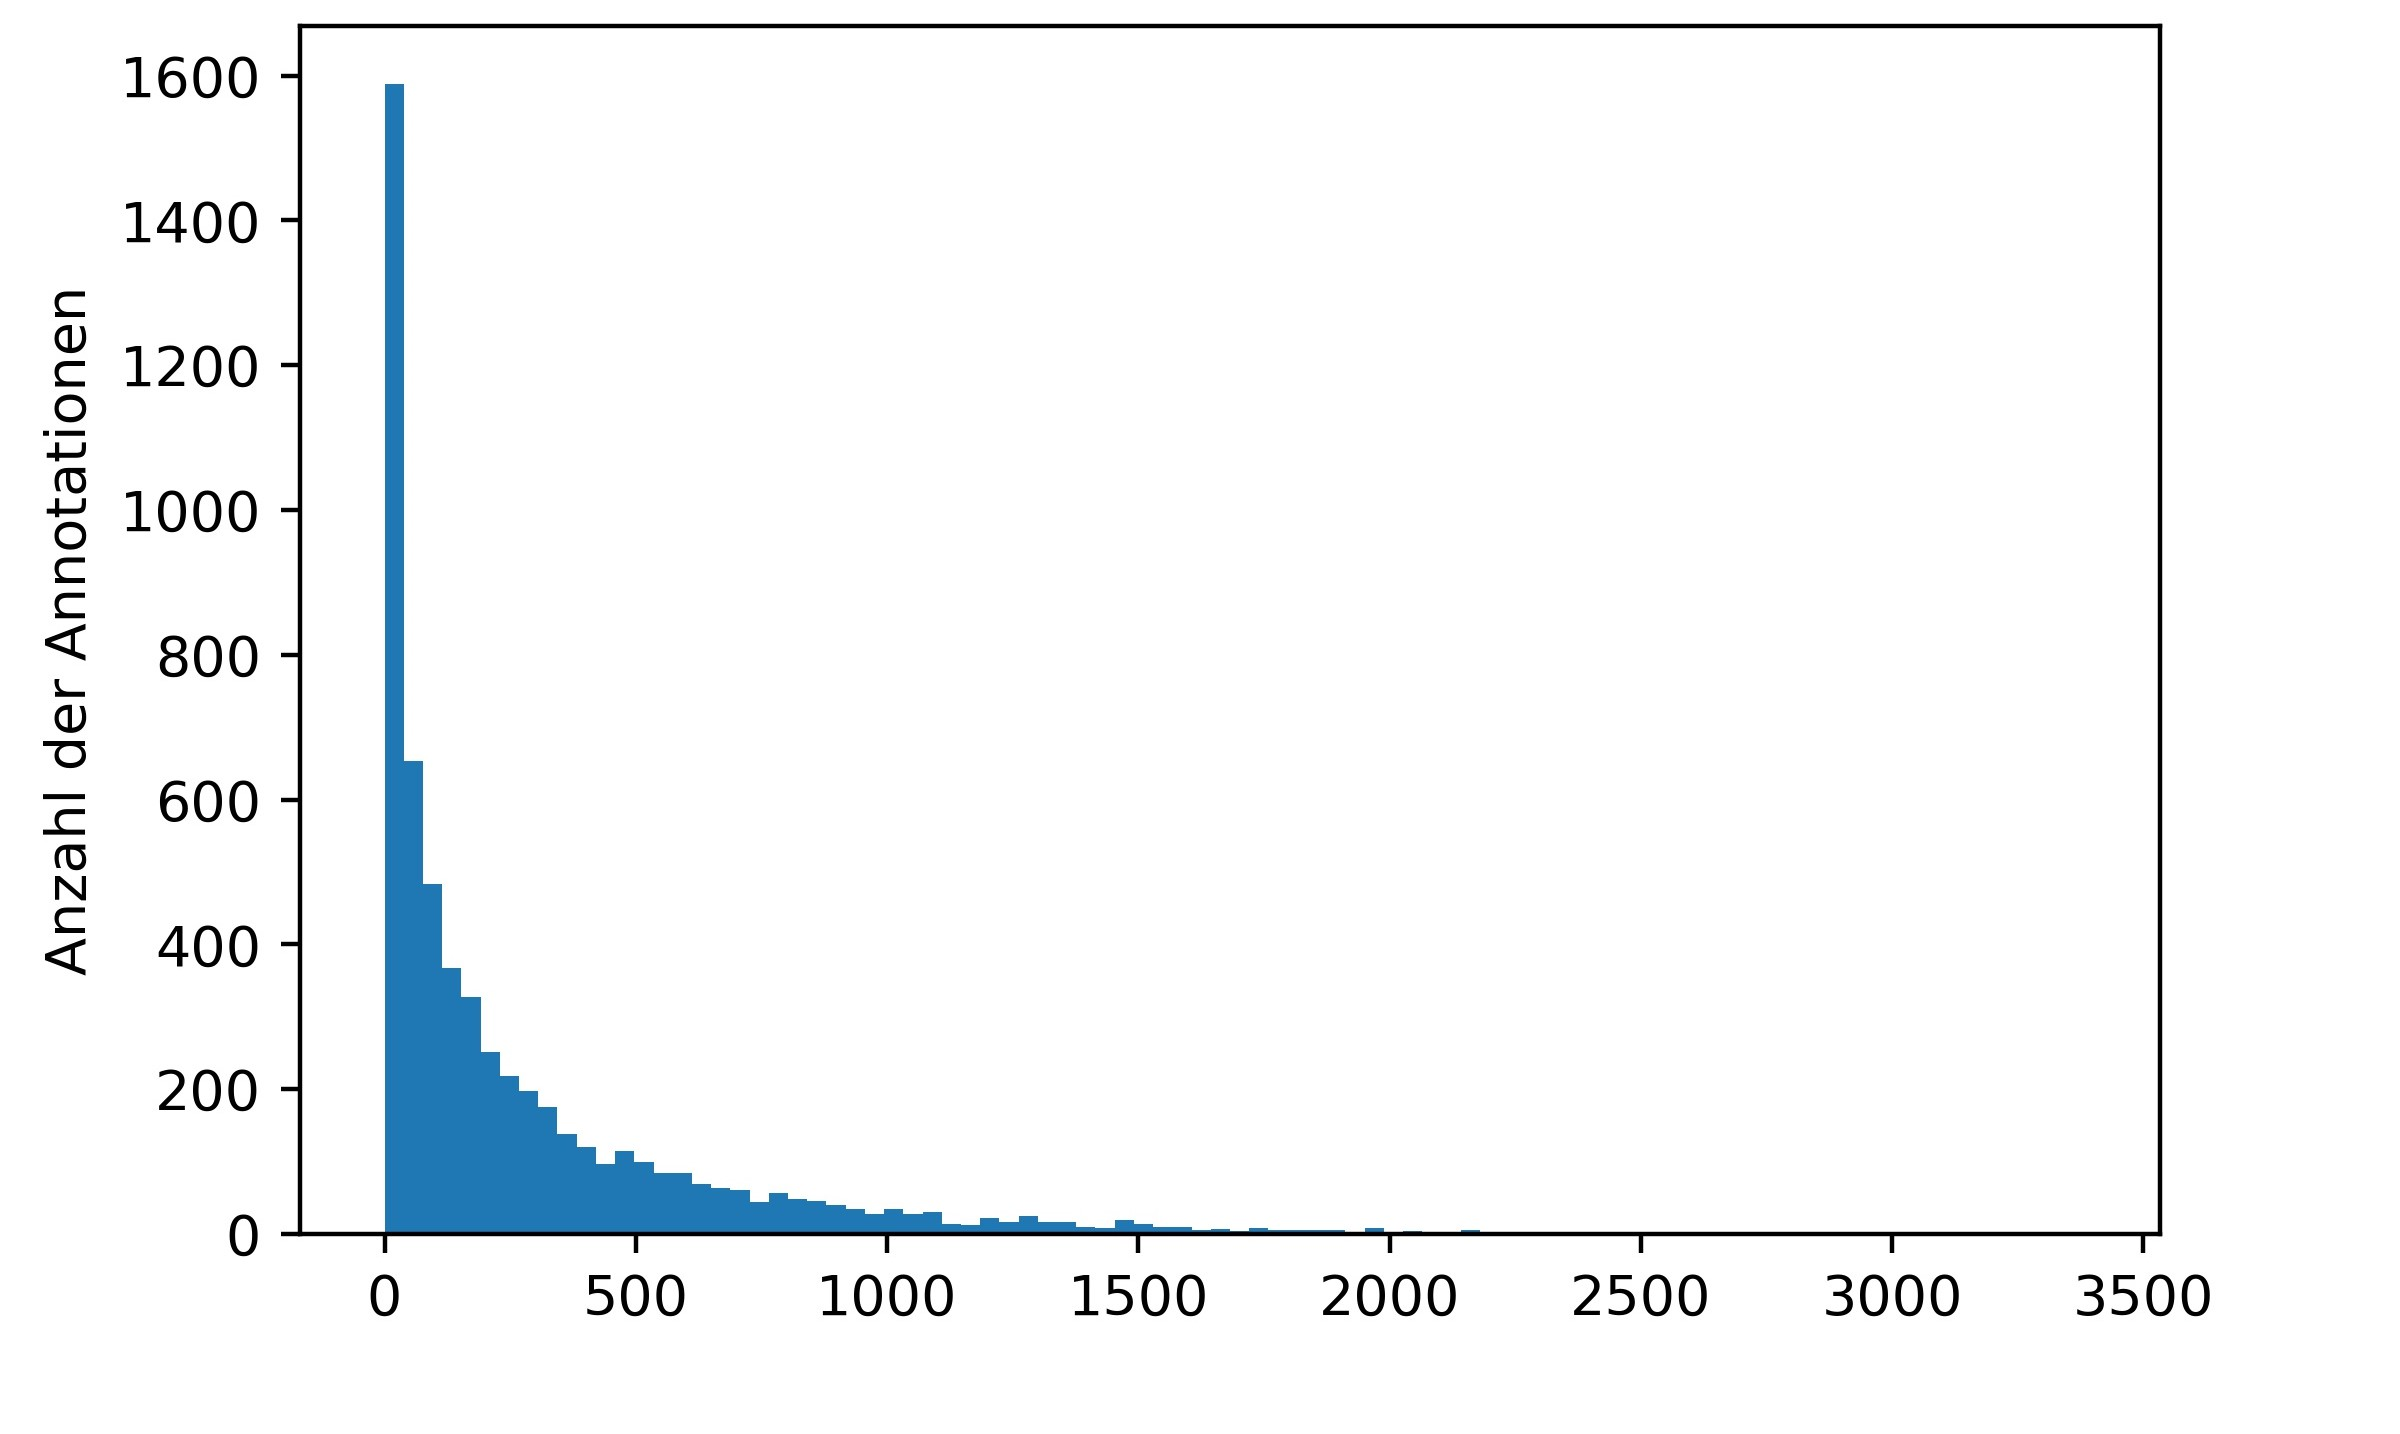
\includegraphics[width=0.80\textwidth]{./Bilder/absolute Kosten.jpg}
		\caption{Histogrammm der absoluten Kosten}
	\end{subfigure}
	\begin{subfigure}[t]{.49\linewidth}%
		\centering
		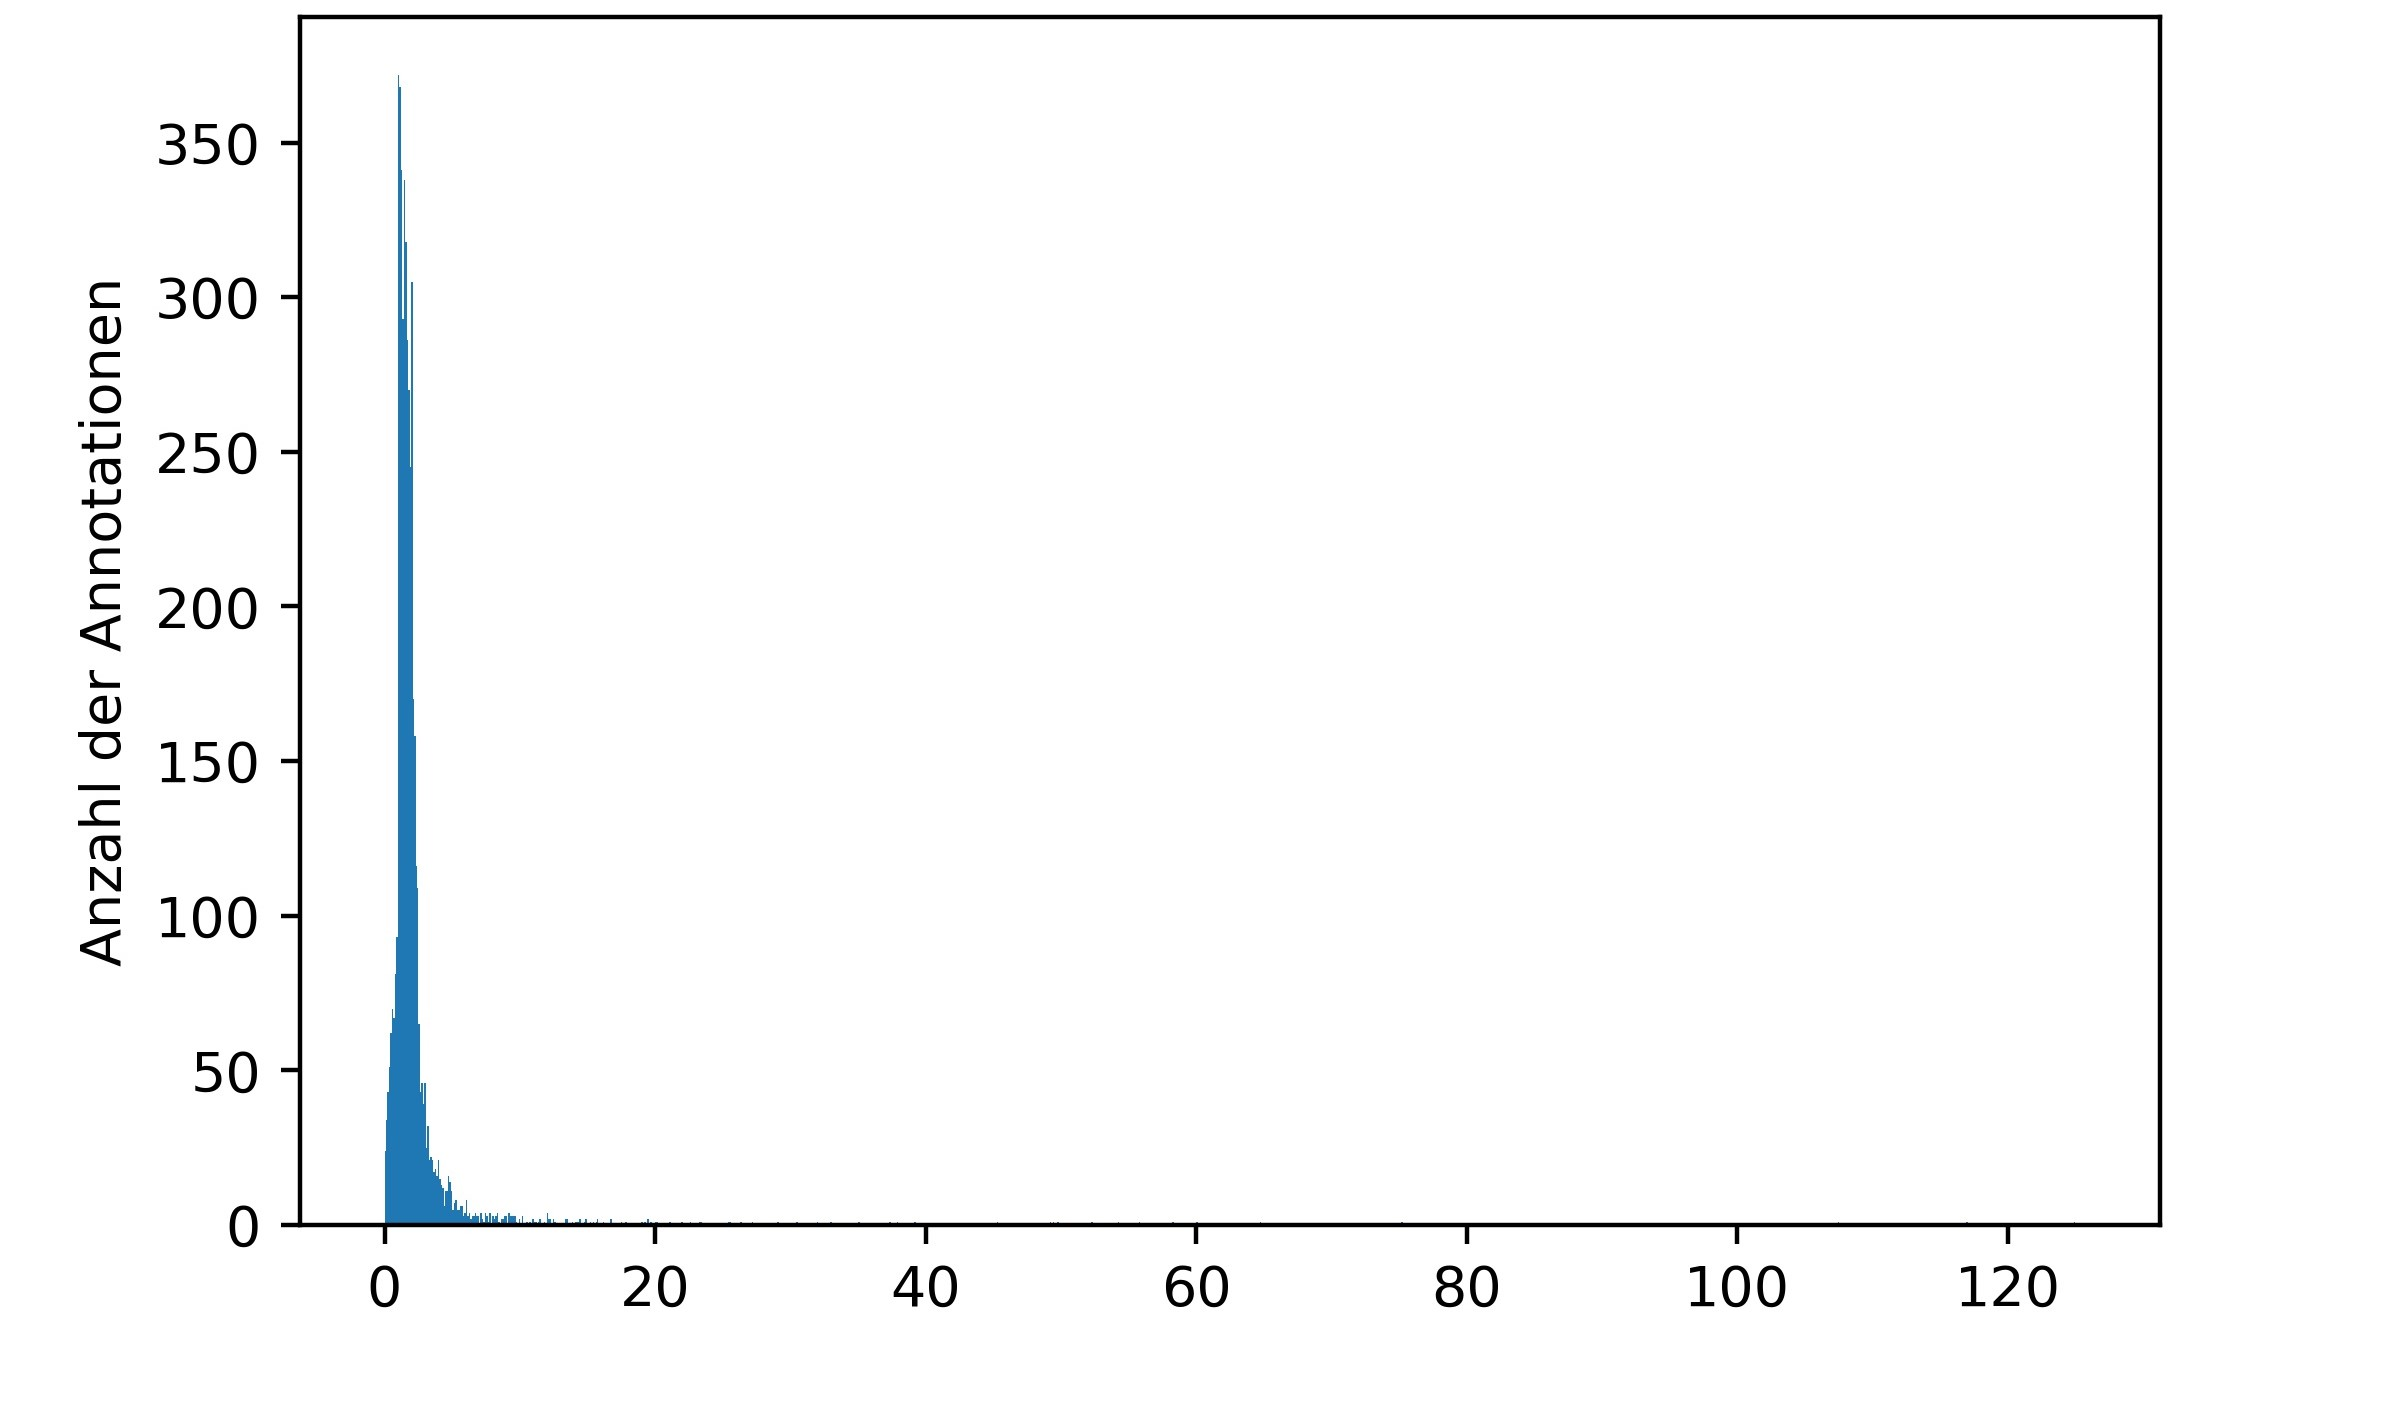
\includegraphics[width=0.8\textwidth]{./Bilder/relative Kosten.jpg}
		\caption{Histogrammm der relativen Kosten}
	\end{subfigure}
\caption{Darstellung der Kostenverteilung mit einer automatisch erstellten Balkenweite}
\label{fig:Kostennebeneinander}
\end{figure}



\section{Verbesserung der Einordnung des Detektors}
Die Metriken zu Verbesserung der Einordnung des Detektors sind in Tabelle \ref{tab:VerbesserungMetriken} zu sehen. Der Anhang "mean" beschreibt den Mittelwert der Verteilung über die Differenz der Start- oder Endzeitpunkte von TP. Die Anhand "std" beschreibt analog die Standardabweichung der Verteilung.
\begin{table}[!ht]
\caption{Metriken aus dem Kapitel \ref{Verbesserung}: "Verbesserung der Einordnung des Detektors"}
	\centering
		\begin{tabular}{lll}
			\hline & Mittelwert & Median\\
			\hline {$\!\begin{aligned}
				&\\
				Falsch\ positiv\ Rate\\
    			Verstö"se\ gegen\ die\ LM-Zeitkriterien\\
				Anzahl\ der\ Xto1-Matches\\
				Anzahl\ der\ 1toX-Matches\\
    			Schwerpunkt\\
		        LM-Anzahl\ (automatisch\ / \ manuell)\\
				Startzeitpunkte_{mean}\\
				Startzeitpunkte_{std}\\
				Endzeitpunkte_{mean}\\
				Endzeitpunkte_{std}\\
			
				&\\
				\end{aligned}$} & {$\!\begin{aligned}
				&\\
				0.55\\
				0\\
				2.9\\
				1.6\\
				136\ Sekunden\\
				1.6\\
				-0.38\ Sekunden\\
				0.83\ Sekunden\\
				0.76\ Sekunden\\
				1.2\ Sekunden\\
				&\\
				\end{aligned}$} & {$\!\begin{aligned}
				&\\
				0.56\\
				0\\
				0\\
				0\\
			    50\ Sekunden\\
				0.89\\
				-0.26\ Sekunden\\
				0.67\ Sekunden\\
				0.64\ Sekunden\\
				1\ Sekunde\\
				&\\
				\end{aligned}$}\\
				\hline
		\end{tabular}

\label{tab:VerbesserungMetriken}
\end{table}

Zur besseren Einordnung der LM Verhältnisse wurde die Differenz der Anzahl zwischen automatisch und manuell annotierten LM berechnet. Der Mittelwert beträgt -87.1. Da das Vorzeichen negativ ist, wurden im Mittel mehr manuelle LM annotiert.


Das Histogramm über alle Schwerpunktdifferenzen ist in Grafik \ref{fig:centers} dargestellt. Es sind keine Teilmengen im Histogramm zu erkennen, die die Festsetzung eines Schwellwertes erlauben würden.
\begin{figure}[!ht]%
	\begin{center}
	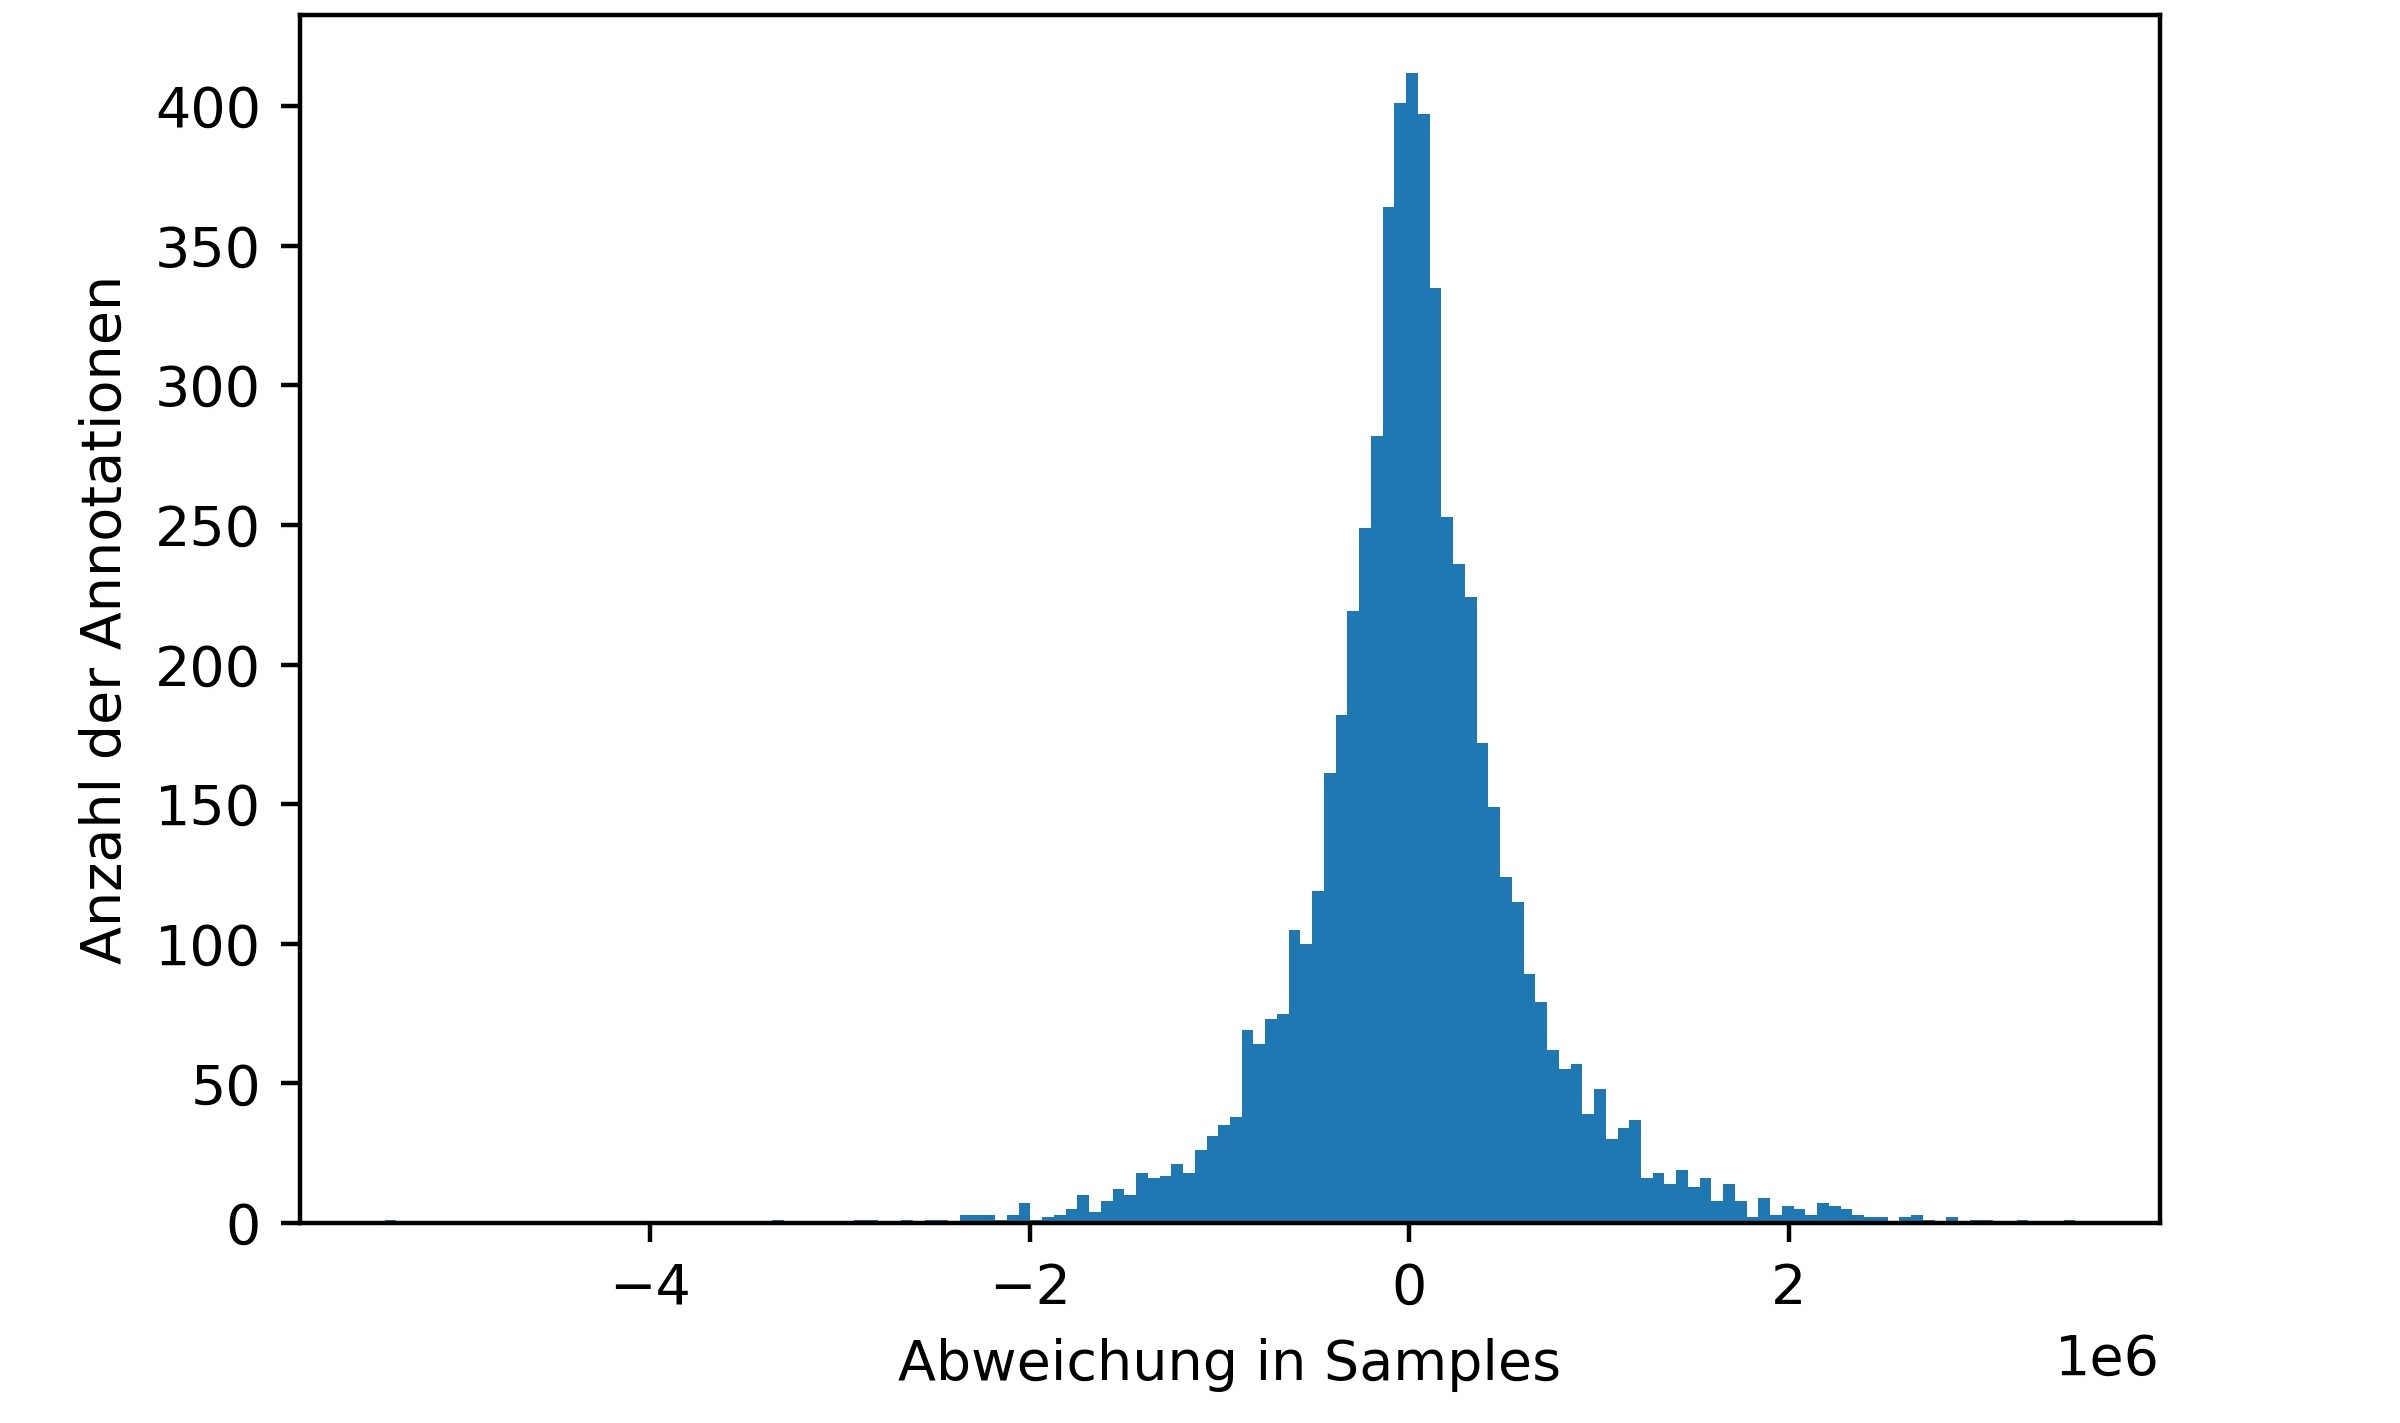
\includegraphics[width=0.80\textwidth]{./Bilder/centers.jpg}
	\end{center}
	\caption{Histogramm über die Differenz der Schwerpunkte aus automatischer und manueller Annotation. Die Breite der Balken wurde für die gesamte Arbeit automatisch erstellt.}%
	\label{fig:centers}%
\end{figure}

Dieses Histogramm zeigt die falsch positiv Rate. Die Häufung um den Wert 0.5 deutet darauf hin, dass FP und TN ähnlich häufig vorkommen. In dem Histogramm sind nur die Dateien mit ohne FP auffällig als eigenständige Teilmenge.

\begin{figure}[!ht]%
	\begin{center}
	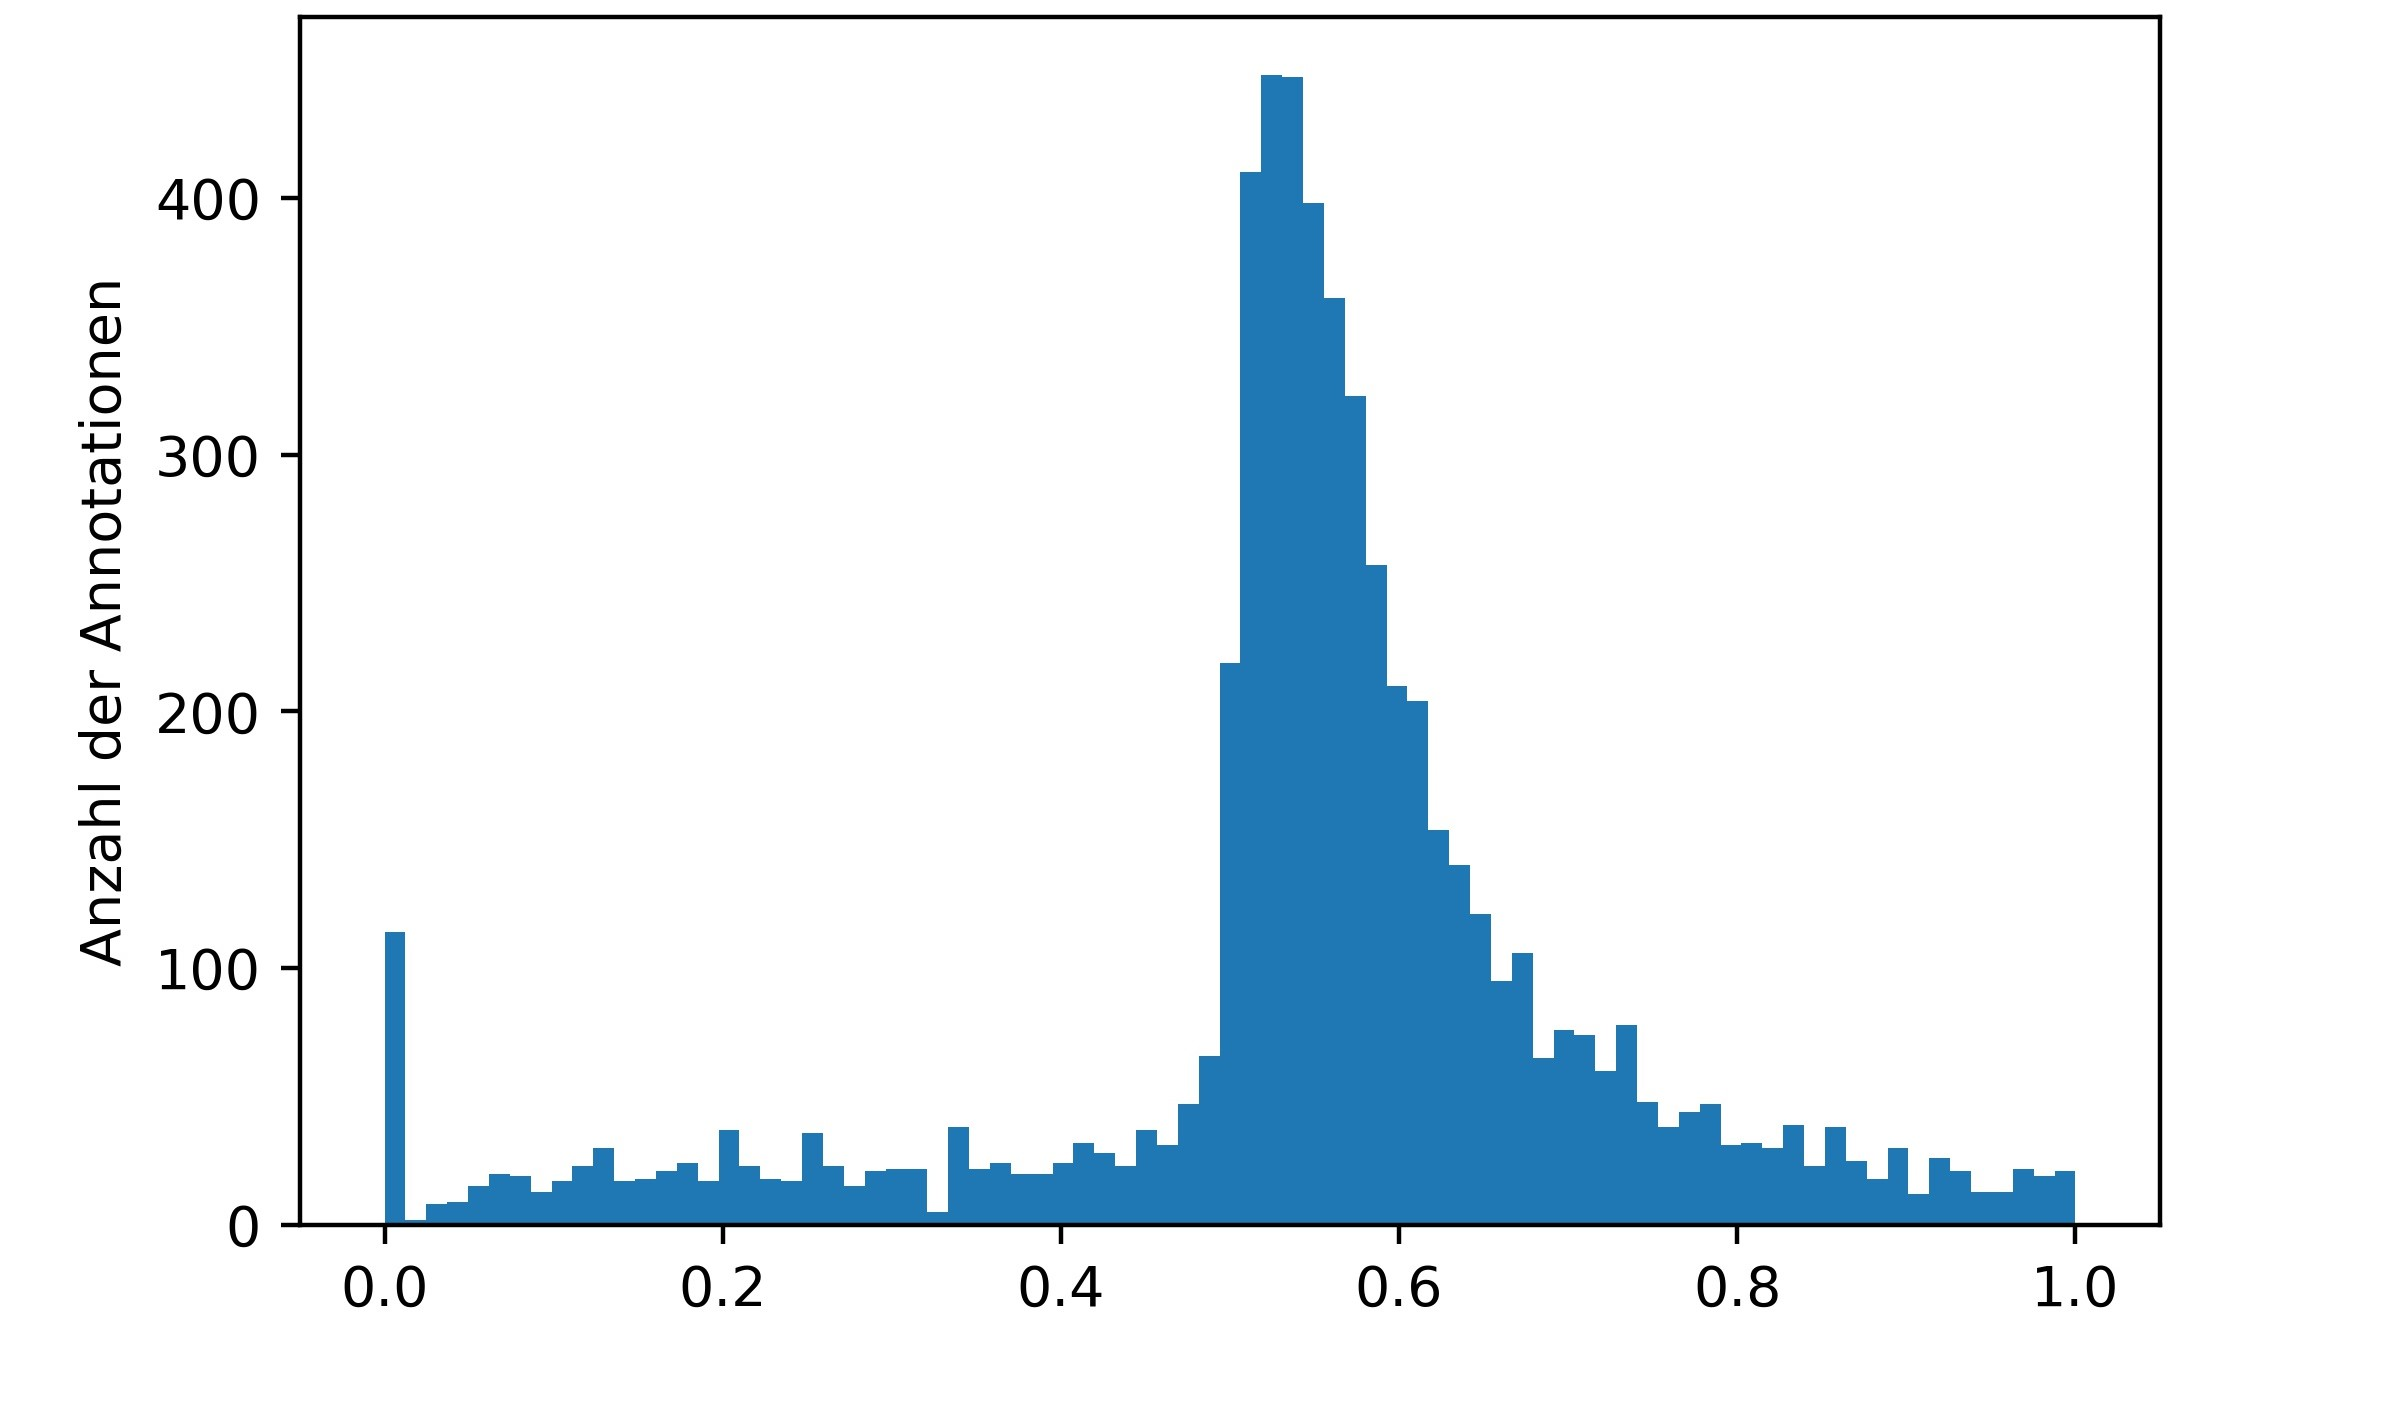
\includegraphics[width=0.80\textwidth]{./Bilder/falsch positiv Rate.jpg}
	\end{center}
	\caption{Histogramm über die falsch-positiv Rate. Die Breite der Balken wurde automatisch erstellt.}%
	\label{fig:FPrate}%
\end{figure}
